\section{N-BRW WITH LIGHT TAILS}\label{sec:light_tails}

In \cite{exp_tails} Bérard and Gouéré studied the $N$-BRW whose point process is given by two independent draws from a distribution $p$ that has finite moment generating function in some neighbourhood of zero and whose spine can be centred (see \ref{eqn:t*exists}). In this section we adapt their results to the more general case of $N$-Branching Random Walks with finite logarithmic moment generating function in a neighbourhood of zero whose spine can be centered. Loosely speaking we extend their results to the case where the number of offspring are random and their position not necessarily independent of each other. We use the methods of \cite{exp_tails} for most proofs, adding details and adapting the arguments as necessary. 

\subsection{The model}\label{subsec:The_model}
Consider the BRW $(\widehat{\bb{T}}, \widehat{V})$ governed by the point process $\widehat{\scr{L}}$ with logarithmic moment generating function $\widehat{\psi}$. Assume that (\ref{eqn:TreeAssumptions}), (\ref{eqn:t*exists}) and (\ref{ass:DacyingTails}) holds. Let $(\widehat{X}_n)_{n \geq 0}$ be the corresponding $N$-BRW and write $\max \widehat{X}_n$ and $\min \widehat{X}_n$ for the position of the right- and leftmost particle of $\widehat{X}_n$. We will show that 
\begin{equation}\nonumber
\hat{v}_N \defeq \lim_{n \to \infty} n^{-1}\max\widehat{X}_n = \lim_{n \to \infty} n^{-1}\min\widehat{X}_n
\end{equation} 
exists in $L^1$ and almost surely. The main result in this section is the analogue of Theorem 1 of \cite{exp_tails}: 
\begin{theorem}\label{thm:ExpTails_BrunDer_non_transformed}
As $N$ goes to infinity, 
\begin{equation}\nonumber
\widehat{v}_N = \widehat{\psi}'(t^*) - \frac{\pi^2 t^* \widehat{\psi}''(t^*)}{2 (\log N)^2} + o((\log N)^{-2}). 
\end{equation}
\end{theorem}


% Notice that if instead of $\widehat{\scr{L}}$ we used the point process $\widehat{\scr{L}}_N$ defined as $\widehat{\scr{L}}_N \defeq \sum^{N \land \# \scr{L}}_{i=1} \delta_{\scr{L}(i)}$ the resulting $N$-BRW would be exactly the same. Since $\# \widehat{\scr{L}}_N \leq N$ almost surely we see that assumption (\ref{ass:killed_assumption_Lp}) can be taken for granted. 


It will be more convenient to work with the BRW that is obtained after the transformation (\ref{eqn:transformation}). The resulting BRW will be denoted by $(\bb{T}, V)$ with point process $\scr{L}$ and logarithmic moment generating function $\psi$ that satisfies (\ref{eqn:BRW_V_Ass}). Observe that the associated random walk $(S_n)_{n \geq 0}$ with step distribution $X$ then satisfies (\ref{eqn:RWCentred}), i.e. $\E X = 0$. Let $X \defeq (X_n)_{n \geq 0}$ denote the $N$-BRW with point process $\scr{L}$ and take $X_0 \in \frak{M}_N$ deterministic. Assuming they exists, $v_N \defeq \lim_{n \to \infty} n^{-1} \max X_n$ is related to $\hat{v}_N$ by 
\begin{equation}\label{eqn:speed_relation}
v_N + \widehat{\psi}(t^*)= \hat{v}_N t^*, 
\end{equation}
as can be seen from (\ref{eqn:transformation2}). Therefore, what we will prove the following:
\begin{theorem}[Brunet-Derrida behaviour, centred form] \label{thm:ExpTails_BrunDer}
As $N$ goes to infinity, 
\begin{equation}\nonumber
v_N = - \frac{\pi^2 (t^*)^2 \widehat{\psi}''(t^*)} {2 (\log N)^2} + o((\log N)^{-2}). 
\end{equation}
\end{theorem}

\subsection{Properties of the model}
Clearly for all $t\in\R$ and $k \geq 1$ we have 
\begin{equation}\nonumber
0 \leq e^{t\, \scr{L}_{n,j}(k)} \leq \sum_{|x|=1} e^{t\, V(x)}
\end{equation} so by assumption (\ref{ass:DacyingTails}) the $\scr{L}_{n,j}(k)$ have finite moment generating function in a neighbourhood of zero which implies exponentially decaying tails. It follows by Lemma \ref{lem:ExpTailsMax} that $\min X_n$ and $\max X_n$ are integrable and hence finite almost surely. Let $d(X_n) \defeq \max X_n - \min X_n$ be the diameter of $X_n$. The following result is analogous to Corollary 1 of \cite{exp_tails} and says that the diameter doesn't get too large:

\begin{proposition}\label{prop:diameter}
For any $N \geq 1$ and initial population $X_0 \in \frak{M}_N$, we have 
\begin{equation}\nonumber
\frac{d(X_n)}{n} \xrightarrow[n \to \infty]{a.s.,\, L^1} 0. 
\end{equation}
\end{proposition}

\begin{remark}
In \cite{mallein2018n} Mallein shows something stronger: he shows that there exists $C > 0$ such that for all $N$, 
\begin{equation}\nonumber
\Pr{d(X_n) > y} \leq C \left( \frac{N(\log N + \log y)}{y}\right)^2
\end{equation}
for all sufficiently large $n$. Using this we can get an upper bound on $\E\, d(X_n)$:
\begin{equation}\nonumber
\E\, d(X_n) = \int\limits_0^\infty \Pr{d(X_n) > x} dx \leq 1 + C N^3 \int\limits^\infty_N \left[\frac{\log x}{x}\right]^2 dx = 1 + C N^2[ \log^2 N + 2 \log N + 2]. 
\end{equation}
\end{remark}

\begin{wrapfigure}{R}{0.5\textwidth}
\centering
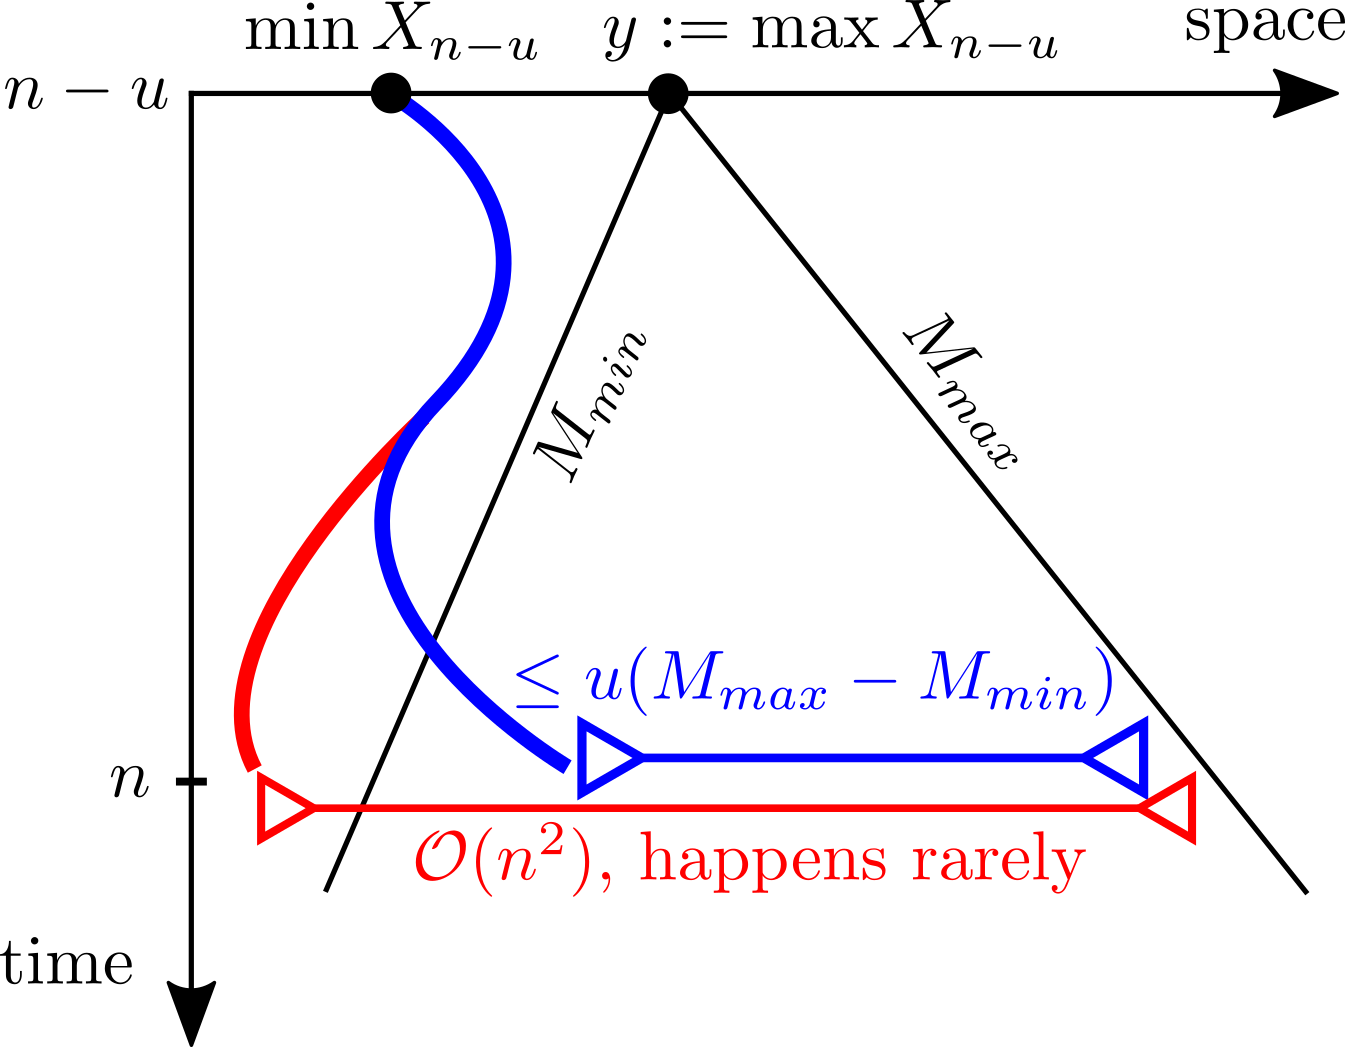
\includegraphics[width=0.45\textwidth]{graphics/g2.png}
% \caption{\label{fig:frog1}This is a figure caption.}
\end{wrapfigure}

\begin{proof}[Proof of Proposition \ref{prop:diameter}]
Let $u \in \N_+$ and for $n \geq u$ consider the process $X$ in the timeframe $\bbracket{n - u, n}$. Define 
\begin{align*}
M_{min} &\defeq \min\{ \scr{L}_{i, j}(N) \mid\, i \in \bbracket{n-u, n-1},\, j \in [N]\} \\
M_{max} &\defeq \max\{ \scr{L}_{i, j}(1) = \max\scr{L}_{i,j} \mid\, i \in \bbracket{n-u, n-1},\, j \in [N]\}
\end{align*} 
to be the smallest respectively largest random walk steps made between times $n-u$ and $n$. By Lemma \ref{lem:ExpTailsMax} both $M_{min}$ and $M_{max}$ are integrable. Write $y \defeq \max X_{n - u}$ for the rightmost particle's position at time $n-u$. \\

Suppose that for each $k \in [u]$ we have $\min X_{n - u + k} < y + k m$. As all steps during branching are $ \geq M_{min}$, this implies in particular that the descendants of the particle at space-time point $(y, n-u)$ survive all selection steps until time $n$. Consider a Galton-Watson process $G \defeq (G_n)_{n \geq 0}$ with offspring distribution $\scr{L}$ coupled with the descendants of $(y, n-u)$ and consider the event $A_u \defeq \{ G_u > N\}$. Since $\Ex{\#\scr{L}} > 1$ and $\#\scr{L} \geq 1$ almost surely, $\Pr{A_u} \to 1$ as $u \uparrow \infty$ where $\Pr{A_u}$ is independent of $n$. Since at most $N$ descendants of $y$ can be alive at any time, on $A_u$ we must have $\min X_{n - u + k} \geq y + k_0 M_{min}$ for some $k_0$. By the definition of $M_{min}$ this must also hold for all $k \in \bbracket{k_0, u}$, in particular for $k = u$. Noting that $\max X_n \leq y + u M_{max}$, it follows that 
\begin{equation}\label{eqn:ExpTailDiamUpperBound}
d(X_n)\Ind_{A_u} \leq u (M_{max} - M_{min}), 
\end{equation}
with probability one. Fix $\epsilon > 0$ and take $u$ large enough so that $\Pr{A_u^c} < \epsilon^2$ and consider the decomposition
\begin{equation}\label{eqn:ExpTailsDiamDecomp}
\frac{d(X_n)}{n} = \frac{d(X_n)}{n} \Ind_{A_u} + \frac{d(X_n)}{n} \Ind_{A_u^c}. 
\end{equation}
Taking expectations and then taking $n$ to infinity, the first term vanishes by (\ref{eqn:ExpTailDiamUpperBound}). The second term is upper bounded by $(\Pr{A_u^c} \Ex{d(X_n)^2 / n^2})^{1/2}$ using Hölder's inequality. A rough bound on $d(X_n)$ suffices: $d(X_n)$ is stochastically dominated by the sum of $n$ i.i.d. copies of $\max_{j \in [N]} \scr{L}_{0, j}(1) - \min_{j \in [N]} \scr{L}_{0,j}(N)$. Since the $\scr{L}_{n,j}(k)$ have exponentially decaying tails, by Lemma \ref{lem:ExpTailsMax} this yields $\Ex{d(X_n)^2} = \cal{O}(n^2)$ which implies that the second term in \ref{eqn:ExpTailsDiamDecomp} is $\cal{O}(\epsilon)$. Taking $\epsilon$ to zero concludes the proof of $L^1$ convergence. Almost sure convergence is a consequence of the proof of the next Proposition. 
\end{proof}

The original proof of Bérard and Gouéré is identical to ours up to the point where we consider the Galton Watson process $G$. Since they only considered binary BRWs, for $u > \log_2 N$ it is clear that $\Pr{A_u} = 1$ so that there is no need to decompose, they just conclude $d(X_n) \leq u(M_{max} - M_{min}$ almost surely. 

\begin{proposition}[{{\cite[Proposition 2]{exp_tails}}}]\label{prop:ExpTailsSpeedExistence}
There exists $v_N \in \R$ such that for any initial population $X_0 \in \frak{M}_N$ the following holds almost surely and in $L^1$:
\begin{equation}\nonumber
\lim\limits_{n \to \infty} \frac{\min X_n}{n} = \lim\limits_{n \to \infty} \frac{\max X_n}{n} = v_N. 
\end{equation}
\end{proposition}

\begin{proof}
First we treat the case $X_0 = N \delta_0$. Recall the definition of $(\scr{L}_{n, j})_{n \geq 0, j \in [N]}$ from the construction of $X$. For each $l \geq 0$ we define the process $(X^r_n)_{n \geq 0}$ by shifting the origin of time by $r$. More precisely, $X^r_0 = N \delta_0$ for each $r \geq 0$ and given the process up to time $n \geq 0$, $X^r_{n+1}$ is be given by the $N$ rightmost particles of 
\begin{equation}\nonumber
\sum_{j = 1}^N \sum_{l \in \scr{L}_{r + n + 1, j}} \delta_{X^r_n(j) + l}. 
\end{equation}
It is clear that given their initial state, $((X^r_n)_{n \geq 0})_{r \geq 0}$ are identically distributed. In particular, $(X^0_n)_{n \geq 0} = (X_n)_{n \geq 0}$ almost surely. From Lemma \ref{lem:monotonicity} it follows easily that 
\begin{equation}\label{eqn:subadd}
\max X^0_{n + m} \leq \max X^0_n + \max X^n_m \qquad \forall\, n,m \geq 0. 
\end{equation}
For clarity define $Z_{i,j} = \max X^i_{j - i}$ for $0 \leq i \leq j$. Then (\ref{eqn:subadd}) reads $Z_{0, j} \leq Z_{0,i} + Z_{i,j}$ for all $0 \leq i \leq j$, which is familiar territory for Kingman's Subadditive Ergodic Theorem. We postpone showing that the conditions of the theorem hold to Lemma \ref{lem:ExpTailsKingmanHolds}. Applying Kingman's Subadditive Theorem yields 
\begin{equation}\nonumber
\lim_{n \to \infty} n^{-1} \max X_n = \lim_{n \to \infty} \Ex{n^{-1} \max X_n} = \inf_n \Ex{n^{-1} \max X_n} = v_N \in \R
\end{equation}
where the first limit is almost sure. Noting that the process $(-X_n)_{n \geq 0}$ also satisfies the hypothesis of the theorem by our assumptions, we can deduce from the identity $\min X_n = - \max (-X_n)$ that 
\begin{equation}\nonumber
\lim_{n \to \infty} n^{-1} \min X_n = \lim_{n \to \infty} \Ex{n^{-1} \min X_n} = \inf_n \Ex{n^{-1} \min X_n} = \tilde{v}_N \in \R
\end{equation}
exists too, where the first limit is almost sure. From the proof of Proposition \ref{prop:diameter} we immediately get $\tilde{v}_N = v_N$ by uniqueness of $L^1$ limits, which gives $\lim_{n\to\infty} n^{-1}d(X_n) = v_N - \tilde{v}_N = 0$ almost surely as claimed in the previous proposition. The proof is complete in the case $X_0 = N \delta_0$. By translation invariance of the dynamics of the system the result also follows for initial states of the form $N \delta_{x_0}$ for any $x_0 \in \R$. Finally, for arbitrary $X_0 \in \frak{M}_N$ note that the result is a consequence of Lemma \ref{lem:monotonicity} and a sandwiching argument between the initial states $N \delta_{\min X_0}$ and $N \delta_{\max X_0}$. 
\end{proof}

\begin{wrapfigure}{R}{0.5\textwidth}
\centering
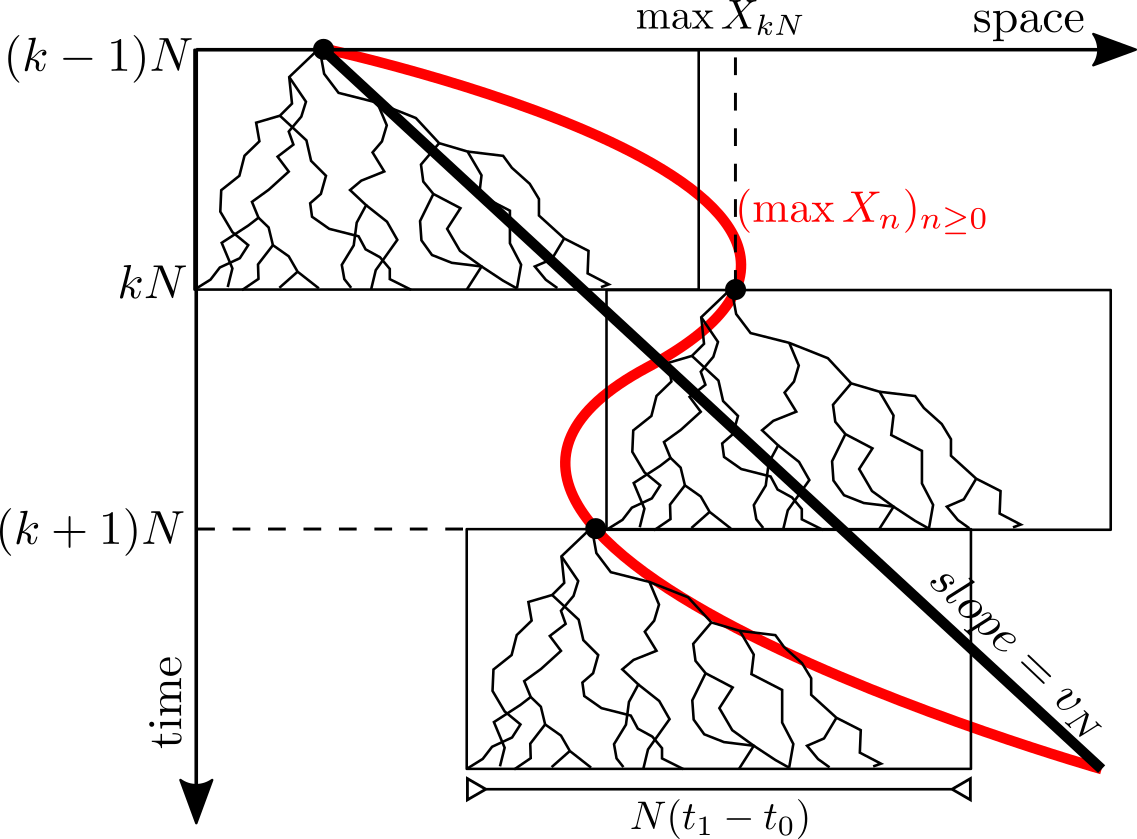
\includegraphics[width=0.45\textwidth]{graphics/g1.png}
% \caption{\label{fig:frog1}This is a figure caption.}
\end{wrapfigure}

Inspecting the previous proof, we see that the existence of $v_N$ and $\tilde{v}_N$ (the almost sure and $L^1$ limits of the left- and rightmost particles) when started from $X_0 = N \delta_0$ was shown without relying on Proposition \ref{prop:diameter}. We can in fact deduce Proposition \ref{prop:diameter} by an argument inspired by one of Prof. Berestycki's suggestions:

\begin{proof}[Alternative proof of Proposition \ref{prop:diameter}]
Let $Y = (Y_n)_{n \geq 0}$ be a branching random walk (without selection) with point process $\scr{L}$. Start $Y$ from $\delta_{0}$ noting that initially there is only one particle. Since $\Ex{\# \scr{L}} > 1$ by assumption, the probability $\rho_1$ that the number of particles in $Y$ has reached $N$ by time $N$ is strictly positive. Define $M_{min}$ and $M_{max}$ for $Y$ analogously to their definition in the proof of Proposition \ref{prop:diameter}. By Lemma \ref{lem:ExpTailsMax} one can find $t > 0$ large enough such that $\rho_2 \defeq \PrCond{-t \leq m_Y \leq M_Y \leq t }{\# Y_N \geq N} > 0$. We can now write

\begin{align*}
\Pr{\{ \# Y_N \geq N \} \cap \{-t \leq m_Y \leq M_Y \leq t \}} &= \Pr{\# Y_N \geq N} \PrCond{-t \leq m_Y \leq M_Y \leq t }{\# Y_N \geq N} \\
															   &\geq \rho_1 \rho_2 > 0. 
\end{align*}
Suppose that we couple $X$ with independent copies of $Y$  placed at the space-time points $(\max X_{kN}, kN)_{k \geq 0}$ denoted by $((Y^{(k)}_n)_{0 \leq n \leq N})_{k \geq 0}$. By the second Borel-Cantelli lemma it follows that almost surely infinitely many of the $(Y^{(k)}_n)_{0 \leq n \leq N}$ must have $N$ particles by time $N$ and have $-t \leq m_Y \leq M_Y \leq t $. This in turn implies that for infinitely many $k \geq 0$ the diameter is less than $2Nt$ for some time $n \in [Nk, N(k+1))$. This immediately yields $\tilde{v}_N = v_N$. 
\end{proof}

\begin{proposition}[{{\cite[analogue of Proposition 3]{exp_tails}}}]\label{prop:increasing_speed}
The sequence $(v_N)_{N \geq 1}$ is non-decreasing. 
\end{proposition}
\begin{proof}
This is again a consequence of Lemma \ref{lem:monotonicity}. 
\end{proof}

% \begin{remark}\label{rem:constants}
% From Proposition \ref{prop:increasing_speed} we can deduce that $v_N$ increases to a possibly infinite limit $v_\infty$ as $N$ goes to infinity. Assumption \ref{ass:exponential_tails} implies that $\Lambda$ is smooth on the interior of $\cal{D}(\Lambda)$ so that both quantities $v \defeq \psi'(t^*)$ and $\chi \defeq \frac{\pi^2}{2} t^* \psi''(t^*)$ are finite. In Section \ref{sec:ExpTails_BrunDer} we will see that $v_\infty$ is in fact equal to $v$. 
% \end{remark}





\subsection{Brunet-Derrida behaviour}\label{sec:ExpTails_BrunDer}
First let us describe the coupling between the $N$-branching random walk and $N$ independent branching random walks which allows us apply Theorems \ref{thm:infty_good} and \ref{thm:finite_good}. Let $(\text{BRW}_j)_{j \in [N]} = ((\bb{T}_j, V_j))_{j \in [N]}$ be $N$ independent copies of the BRW with point process $\scr{L}$. Define $\scr{T}_n \defeq \bigsqcup_{j=1}^N \{ x \in \bb{T}_j \,:\, |x|=n \}$ to be the disjoint union of vertices at depth $n$. We now inductively define a sequence $(G_n)_{n \geq 0}$ of random subsets of $\scr{T}_n$, each with exactly $N$ elements. These random subsets will correspond to the particles alive in the coupled $N$-braching random walk at time $n$. Define $G_0 = \scr{T}_0$ and given $G_n$, define $H_n$ to be the vertices in $\scr{T}_{n+1}$ that descend from vertices in $G_n$. Finally, set $G_{n+1}$ to be the set of $N$ vertices in $H_n$ with the gratest value. If we now define (with some abuse of notation) $\frak{X}_n = \sum_{u,j : u \in G_n \cap \bb{T}_j} \delta_{V_j(u)}$ then $(\frak{X}_n)_{n \geq 0}$ has the same distribution as $X$ started from $N \delta_0$. 
% In what follows we will refer to all of $\bb{T}$, $\Phi$, $\epsilon_{n,i,j}$ and $\tau_{n,i}$ without explicitly explaining the obvious relationships between these objects. Let us now record a technical lemma that will be used in the proof of the lower bound in Theorem \ref{thm:ExpTails_BrunDer}. 

\subsubsection{Lower bound}
\begin{proof}[Proof of upper bound in Theorem \ref{thm:ExpTails_BrunDer}]
As before, we first treat the case $X_0 = N \delta_0$. For notational simplicity define $\chi = \pi^2 (t^*)^2 \widehat{\psi}''(t^*) / 2$. Our aim is to show $v_N \defeq \lim_{n \to \infty} \Ex{n^{-1} \max X_n} \leq -  \chi / (\log N)^2 + o((\log N)^{-2})$. Recalling the proof of Proposition \ref{prop:ExpTailsSpeedExistence}, we know by subadditivity that
\begin{equation}\label{eqn:ExpTailsSubaddDecomp1}
v_N \leq \frac{\Ex{\max X_n}}{n} \qquad\qquad\forall\, n \in \N. 
\end{equation}
In light of the desired correction term, we decompose (\ref{eqn:ExpTailsSubaddDecomp1}) into
\begin{equation}\nonumber
\Ex{\max X_n} \leq - \frac{\chi}{(\log N)^2} + \Ex{\max X_n \Ind_{\{\max X_n \geq -n \chi (\log N)^{-2} \}}}. 
\end{equation}
However, this is not the exact form of the RHS that we will work with. Let $\gamma \in (0,1)$ and $\epsilon = \epsilon(N)$ whose precise form we will choose later, but will be approximately $\chi (\log N)^{-2}$ as $N \to \infty$. We go on to show that in
\begin{equation}\nonumber
\Ex{\frac{\max X_n}{n}} \leq  - (1 - \gamma)\epsilon + \Ex{\frac{\max X_n}{n} \Ind_{\{\max X_n \geq  -n (1 - \gamma) \epsilon \}}}
\end{equation}
the last term is $o((\log N)^{-2})$. This will yield the desired upper bound on $v_N$ if we take $\gamma \to 0$. We further decompose the problem: for $\delta > 0$ we have
\begin{equation}\nonumber 
\Ex{\frac{\max X_n}{n} \Ind_{\{\max X_n \geq - n (1 - \gamma)\epsilon \}}} \leq \delta\underbrace{\Pr{\frac{\max X_n}{n} \geq -(1 - \gamma)\epsilon }}_{\circled{1}} + \underbrace{\Ex{\frac{\max X_n}{n} \Ind_{\{ \delta n \leq \max X_n \}}}}_{\circled{2}}. 
\end{equation}
First we show that for an appropriate scaling of $\epsilon=\epsilon(N)$ and $n = n(N)$ we have $\circled{1} = o((\log N)^{-2})$. Set $n = \ceil{N^\xi}$ for some $0 < \xi < \gamma$ and $m = m(N) \leq n$ whose exact form we'll specify soon. Let $B$ be the number of vertices in $\sqcup_{i=0}^n G_i$ that are $(m, - \epsilon)$-good with respect to their corresponding BRWs. Let $u_0, u_1, ..., u_n$ be a path in $\bb{T}_{i_0}$ for some $i_0 \in [N]$ such that $u_0 = root_{i_0}$ and $u_n \in G_n$ with $V_{i_0}(u_n) = \max X_n$. In other words, let $BRW_{i_0}$ be the random walk that the rightmost particle of the coupled $N$-branching random walk lives in at time $n$, and let $u_0, ..., u_n$ be the path connecting it to the corresponding root. Define the event $E \defeq \{ \max X_n \geq - n (1 - \gamma)\epsilon \}$, and apply Lemma \ref{lem:ExpTailsGoodSequencesTechnical} to the sequence of real numbers $(V_{i_0}(u_i))_{i \in [n]}$. It follows that on $E$, for any $K > 0$, either one of the random walk steps along the path is $> K$ or $B \geq \frac{\gamma\epsilon}{K + \epsilon}\frac{n}{m} - \frac{K}{K + \epsilon}$. This yields
\begin{equation}\label{eqn:ExpTailsEBound}
\circled{1} = \Pr{E} \leq \Pr{M \geq K} + \Pr{B \geq \frac{\gamma\epsilon}{K + \epsilon}\frac{n}{m} - \frac{K}{K + \epsilon}},  
\end{equation}
where $M \defeq \max \{\max \scr{L}_{l, j} \mid\, l \in \bbracket{0, n - 1},\, j \in [N]\}$. Set $\beta \in (0, \bb{V}(X))$ and let $\theta > 0$ be as in Theorem \ref{thm:finite_good}. Let $\lambda > 0$, and define 
\begin{equation}\nonumber
m \defeq \ceil*{ \left[\frac{2 \theta}{\pi^2}\right]^{3/2} \left( \frac{(1 + \lambda) \log N}{(\bb{V}(X) - \beta)^{1/2}}\right)^3},
\end{equation} 
and $\epsilon \defeq \theta\, m^{-2/3}$. $m$ is carefully chosen so that by Theorem \ref{thm:finite_good}, 
\begin{equation}\label{eqn:ExpTailsProof}
\rho(m, \epsilon) \leq N^{-(1 + \lambda)} 
\end{equation}
for all large $N$. Also let $K = \kappa \log N$ for $\kappa > 0$ and observe that $\frac{\gamma\epsilon}{K + \epsilon}\frac{n}{m} - \frac{K}{K + \epsilon} > 0$ for large enough $N$ independently of $\kappa$. Thus (\ref{eqn:ExpTailsEBound}) turns into
\begin{equation}\nonumber
\circled{1} = \Pr{E} \leq \underbrace{\Pr{M \geq K}}_{\circled{1a}} + \underbrace{\Pr{B \geq 1}}_{\circled{1b}}. 
\end{equation}

$\circled{1a}$: As noted before, $(\max \scr{L}_{i,j})_{i \geq 0, j \in [N]} = (\scr{L}_{i, j}(1))_{i \geq 0, j \in [N]}$ are i.i.d. with common distribution $\max \scr{L}$ and have exponentially decaying tails so that there exists $C, \phi, K_0 > 0$ such that for all $K > K_0$ it holds that $\Pr{\max \scr{L} > K} \leq C \exp(-\phi K)$. By a calculation similar to the proof of Lemma \ref{lem:ExpTailsMax}, for all large enough $\kappa$ we get
\begin{align}
\Pr{M \geq K} &= 1 - (1 - \Pr{\max \scr{L} > K})^{Nn} \leq 1 - (1 - C \exp(-\phi K))^{Nn} \\
			  &= 1 - (1 - C N^{-\phi \kappa})^{Nn} \leq C N^{-\phi \kappa} Nn = C N^{1 + \xi - \phi \kappa}. 	
\end{align} 
Thus, $\Pr{M \geq K} = o((\log N)^{-2})$ for $\kappa > 2/\phi$. \\

$\circled{1b}$: Consider a vertex $u \in \bb{T}_{j_0}$ for some $j_0 \in [N]$ with $|u| \leq n$. The event $\{u \in G_d\}$ is measurable with respect to the sigma algebra generated by the random variables $\{ V_j(v) \mid\, j \in [N],\, v \in \bb{T}_j,\, |v| \leq |u|\}$. On the other hand, the event $\{ u \text{ is }(m, - \epsilon) \text{-good}\}$ is determined by the variables $\{ V_{j_0}(v) - V_{j_0}(u) \mid\, v \in \bb{T}_{j_0},\, |u| < |v| \}$, so that the two events are independent. We can write $B$ as 
\begin{equation}\nonumber
B = \sum\limits_{i=1}^N \sum\limits_{u \in \bb{T}_i} \Ind_{\{u \text{ is } (m, - \epsilon)\text{-good}\}} \Ind_{\{u \in G_d \text{ for some d} \leq n \}}. 
\end{equation}
Taking expectations gives 
\begin{equation}\nonumber
\Ex{B} \leq N(n+1)\rho(m, \epsilon) = \cal{O}(N^{\xi -\lambda}) = o((\log N)^{-2}) \qquad\text{as $N$ goes to infinity}, 
\end{equation}
where we used that $G_n$ has $N$ elements for all $n$. Applying Markov's inequality to $B$ and combining with our estimate of $\circled{1a}$ gives $\circled{1} = o((\log N)^{-2})$ as desired. \\

We now turn to showing $\circled{2} = o((\log N)^{-2})$. Consider the obvious inequality $\exp(\max X_n) \leq \sum_{j \in [N]} \sum_{x \in \bb{T}_j : |x| = n} \exp(V_j(x))$. It follows from the Many-to-One lemma that 
\begin{align*}
\Ex{\exp(\max X_n)} \leq N\, \E\sum\limits_{|x| = n} \exp(V(x)) = N. 
\end{align*}
Now apply Lemma \ref{lem:ExpTailBound} with $x = \max X_n$ and $a = \delta n$ and take expectations to get 
\begin{align*}
\Ex{\max X_n \Ind_{\{\max X_n \geq \delta n \}}} &\leq \Ex{\exp(X_n - \delta n / 2)} \leq N \, e^{-\delta n / 2} = o((\log N)^{-2}).
\end{align*}
This concludes the proof of the upper bound: we have shown that for any choice of $\gamma \in (0,1)$, $\beta \in (0, \bb{V}(X))$ and $\lambda > \xi > 0$ we have
\begin{equation}\label{eqn:ExpTailResultTally}
v_N \leq \Ex{\ceil{N^\xi}^{-1} \max X_{\ceil{N^\xi}}} \leq - (1 - \gamma) \frac{\pi^2 (\bb{V}(X) - \beta)}{2 (1 + \lambda)^2(\log N)^2} + o((\log N)^{-2}). 
\end{equation}
Taking $\gamma, \beta, \lambda$ and $\xi$ to zero gives the desired result. 
\end{proof}

Here is a summary of the variables used in the previous proof, collected in a table to ease understanding
\begin{center}
\begin{tabular}{|c|c||c|c|} 
 \hline
 % Variable 	& Definition 			& Variable 	& Definition 								            \\
 $\gamma$ 	& $\in (0, 1)$ 			&	$\bb{V}(X)$		& $2 \chi / \pi^2$		        \\

 $\delta$ 	& $\in (0, \infty)$ 	&  	$\beta$			& $\in (0, \bb{V}(X))$								            \\ 

 $\xi$ 		& $\in (0, \gamma)$ 	&	$\theta$	& as in Theorem \ref{thm:finite_good}			                             \\ 

 $\kappa$	& $\in (0, \infty)$		&	$K$ 				& $\kappa \log N$	                 \\

$\chi$ 			& $\pi^2 (t^*)^2 \widehat{\psi}''(t^*) / 2$ &  $m$ & $\ceil*{ \left[\frac{2 \theta}{\pi^2}\right]^{3/2} \left( \frac{(1 + \lambda) \log N}{(\bb{V}(X) - \beta)^{1/2}}\right)^3}$\\

$\lambda$	& $\in (0, \infty)$ & $\epsilon$ & $\theta\,m^{-2/3}$ \\

$n$ 		& $\ceil{N^\xi}$     & & \\

 \hline
\end{tabular}
\end{center}










\subsubsection{Upper bound}
\begin{proof}[Proof of lower bound in Theorem \ref{thm:ExpTails_BrunDer}]

Let $\lambda, \eta \in (0,1)$ and let 
\begin{equation}\nonumber
\epsilon \defeq \frac{\chi}{(1-\lambda)^2(\log N)^2}. 
\end{equation}
With this choice Theorem \ref{thm:infty_good} gives $\rho(\infty, - \epsilon) = N^{\lambda - 1 + o(1)}$ as $N \to \infty$. Recall now the construction of $(X^r_n)_{n, l \geq 0}$ using $(\scr{L}_{n, j})_{n \geq 0, j \in [N]}$ from the proof of Proposition \ref{prop:ExpTailsSpeedExistence}. Define the random variables $\Gamma_0 \defeq 0$ and $J_0 \defeq 0$ and set $i = 0$. Given $\Gamma_i$ and $J_i$ inductively define $L_{i+1} \defeq n \land \inf\{ k \mid\, \min X^{\Gamma_i}_k \geq -(1+\eta)\epsilon k\}$. Finally, let $\Gamma_{i+1} \defeq \Gamma_i + L_{i+1}$ and $J_{i+1} \defeq J_i + \min X^{\Gamma_i}_{L_{i+1}}$. By Lemma \ref{lem:monotonicity} it follows that 
\begin{equation}\label{eqn:regenTime}
\min X_{\Gamma_i} \geq J_i \qquad\forall\, i \geq 0. 
\end{equation}
Observe now that $\Gamma_{i+1} - \Gamma_i$ is an i.i.d. sequence with common distribution $L \defeq n \land \inf \{ k \mid \min X_k \geq - (1+\eta)\epsilon k\}$. Similarly, the sequence $J_{i+1} - J_i$ is also i.i.d. with common distribution $\min X_L$. The strong law of large numbers gives 
\begin{equation}
\lim\limits_{i \to \infty} \frac{\min X_{\Gamma_i}}{i} = \lim\limits_{i \to \infty} \frac{\min X_{\Gamma_i}}{\Gamma_i} \frac{\Gamma_i}{i} = v_N \E L
\end{equation}
almost surely. However, by (\ref{eqn:regenTime}) we also have
\begin{equation}
\liminf\limits_{i \to \infty} \frac{\min X_{\Gamma_i}}{i} \geq \liminf\limits_{i \to \infty} \frac{J_i}{i} = \Ex{\min X_L}.
\end{equation}
Denote $B \defeq \{ \min X_k < - (1+\eta)\epsilon \text{ for all } k \in [n]\}$ and define the random variable $\Theta_n$ to have the law of $\min \{\min \scr{L}_{i, j} \mid\, j \in [N],\, 0 \leq i \leq n - 1 \}$. Combining the obvious inequalities $\min X_L \geq -(1 + \eta)\epsilon L \Ind_{B^c} + n \Theta_n \Ind_B$ and $1 \leq L \leq n$ with the above bounds we get
\begin{equation}\label{eqn:lowerBdd}
v_N \geq \frac{\Ex{\min X_L}}{\E L} \geq -(1+\eta)\epsilon (1 + n\Pr{B}) - n\Ex{|\Theta_n| \Ind_B}. 
\end{equation}
By Hölder's inequality $\Ex{|\Theta_n| \Ind_B} \leq \sqrt{\Ex{\Theta_n^2}\Pr{B}}$. By Lemma \ref{lem:ExpTailsMax} we know that $\Theta_n$ has exponentially decaying tails, so in particular is square-integrable. To prove the lower bound we only need a suitably strong upper bound on $\Pr{B}$. The remainder of the proof is dedicated to this. \\

Since $1 < \Ex{\#\scr{L}} = \E\sum_{|x|=1} \Ind$, by the monotone convergence theorem we can take $R \in \R$ such that $1 < \E\sum_{|x|=1} \Ind_{\{ V(x) \geq R\}}$. If we let $(M_n)_{n \geq 0}$ be the Galton Watson process started from $M_0 = 1$ with offspring law $\sum_{|x|=1} \Ind_{\{ V(x) \geq -R\}}$ then by Lemma \ref{lem:ExpTailsGW} there exist $\phi > 1$ and $r > 0$ such that $\Pr{M_n \geq \phi^n} \geq r$ for all $n \geq 0$. Define now $s \defeq \ceil{\frac{\log N}{\log \phi}} + 1$ and $m \defeq \ceil{\frac{- Rs}{\eta\, \epsilon}}$ and finally set $n = s + m$. Consider a vertex $u$ at depth $m$ in one of the $BRW_i$. The probability that there are at least $\phi^s$ distinct paths $u \eqdef u_m, ..., u_n$ with $V_i(u_{k+1}) - V_i(u_k) \geq R$ for all $k \in \bbracket{m, n - 1}$ is greater than $r$ by our previous discussion. Recall that the probability of the root being $(m, - \epsilon)$-good is $\rho(m, - \epsilon)$. We see that then the probability of observing a path $root = w_0, ..., w_n$ in $BRW_i$ such that $V_i(w_k) \geq - k \epsilon$ for $k \in [m]$ and $V_i(w_{k+1}) - V_i(w_k) \geq R$ for $k \in \bbracket{m, n-1}$ is at least $\rho(m, - \epsilon) r$. By the choice of $s$ and $m$, such a path must also be $(n,  - (1+\eta)\epsilon)$-good. For $i \in [N]$ define $A_j$ to be the event that $BRW_i$ contains no more than $\phi^s$ distinct $(n, - (1+\eta)\epsilon)$-good paths starting at the root. By independence we get
\begin{equation}
\Pr{\bigcap\limits_{i=1}^N A_i} \leq (1 - \rho(m, \epsilon) r)^N. 
\end{equation}
On the event $B \cap [\cap_{i=1}^N A_i]^c$ one of the $BRW_i$s has $> \phi^s > N$ particles at time $n$ that have stayed to the right of the space time line with slope $ - (1 + \eta)\epsilon$ until time $n$. By definition, on $B$ this implies that there are $> N$ particles alive in the $N$-branching random walk which is impossible. Therefore we must have $B \subset \cap_{i=1}^N A_i$. Using the fact that $\rho(m, - \epsilon) \leq \rho(\infty, - \epsilon) = N^{\lambda - 1 + o(1)}$ and the inequality $1 - x \leq \exp(-x)$ for all $x \in \R$, we get
\begin{equation}\label{eqn:ExpTailsBBound}
\Pr{B} \leq \Pr{\bigcap\limits_{i=1}^N A_i} \leq \exp(-N^{\lambda + o(1)})
\end{equation}
Combining the above estimate of $\Pr{B}$ with (\ref{eqn:lowerBdd}) results in 
\begin{equation}
v_N \geq - \frac{\chi (1 + \eta)}{(1 - \lambda)^2(\log N)^2} + o((\log N)^{-2}). 
\end{equation} 
As $\lambda$ and $\eta$ can be taken arbitrarily small, the desired result follows. 
\end{proof}

\subsection{Discussion}
This section is based in part on \cite{exp_tails} Section 8. Write $v_N$ for the asymptotic speed of the $N$-BRW and $v \defeq \lim_{N \to \infty} v$ for its limit, to which it converges at rate $(\log N)^{-2}$. The proof of the Brunet-Deridda behaviour hinged on the idea that the following two are comparable:
\begin{enumerate}[(a)]
\item \vspace{-1mm} $(BRW_j)_{j \in [N]}$ do not survive killing below the speed $v - \epsilon$
\item \vspace{-3mm} $v_N < v - \epsilon$. 
\end{enumerate}
\vspace{-3mm}
It is intuitively clear why this might be true: if $(a)$ holds then we certainly can't expect the $N$-BRW to propagate faster than $v - \epsilon$ since it is dominated by $(BRW_j)_{j \in [N]}$ through the coupling introduced in section \ref{sec:ExpTails_BrunDer}. Conversely, suppose $(a)$ doesn't hold. Consider the particle in the $N$-BRW at time zero that corresponds to a $BRW_i$ that survives killing. With probability $ \sim 1/N$ the descendants of this particle will survive and form the entirety of the $N$-BRW. If this doesn't happen we can `restart' the argument. After a rougly geometric number of attempts we will succed in which case $(b)$ cannot hold. \\

To make such an argument rigorous we needed to get a handle on the probability of a $BRW$ exhibiting paths of various slopes and lengths near the critical slope $0$; the expectation of the $BRW$'s associated random walk. In \cite{gantert2008asymptotics} they did just that using the Many-to-One lemma and one of Mogulskii's results which accurately describes the probabilitiy of a centred random walk's path to stay in a general space-time region. Loosely speaking they show that on the scale $m \propto \epsilon^{-u}$ for $u \in (0, 3/2]$ we have
\begin{equation}
\log \rho(m, -\epsilon) \propto - \epsilon^{-u/3}\qquad\text{as } \epsilon \downarrow 0. 
\end{equation}
Similarly, they show $\log\rho(\infty, -\epsilon) \propto - \epsilon^{1/2}$ as $\epsilon \downarrow 0$. Using this the convergence rate $(\log N)^{-2}$ can be heuristically deduced: setting $\epsilon_N = v - v_N$ we would expect 
\begin{equation}\label{eqn:speed_scale_heuristic}
\rho(\infty, - \epsilon_N) \propto \frac{1}{N}. 
\end{equation}
To see why, suppose for contradiction that $\rho(\infty, - \epsilon_N) \ll 1_N$. Then with probability close to one none of the $BRW_i$ survive killing which would imply that $v_N$ needs to be slower. Conversely, if we had $\rho(\infty, - \epsilon_N) \gg 1/N$ then with probability close to one at least one of the $BRW_i$ would survive killing, implying that $v_N$ needs to be faster. From \ref{eqn:speed_scale_heuristic} and the asymptotic form of $\rho(\infty, -\epsilon)$ for small $\epsilon$ it follows that for all large $N$, $\epsilon_N$ should satisfy
\begin{equation}
\epsilon_N \propto (\log N)^{-2}. 
\end{equation}

\subsection{$\alpha$-stable spine}

In \cite[Lemma 4.2]{mallein2018n} Mallein studies a generalisation of the model we considered in this section. Recall that if $(\bb{T}, V)$ is a $BRW$ with point process $\scr{L}$ that satisfies (\ref{eqn:BRW_V_Ass}) i.e.
\begin{equation}
e^{\psi(1)} = \E \sum\limits_{|x|=1} e^{V(x)} = 1, 
\end{equation}
then the step distribution of the spine $X$ is given by
\begin{equation}
\Pr{X \leq x} = \E \sum\limits_{|u| = 1} \Ind_{\{V(u) \leq x\}} e^{V(u)}. 
\end{equation}
In Section \ref{sec:light_tails} we considered the case when $X$ had finite mean and variance so that by the central limit theorem it belonged to the domain of attraction of the Gaussian law. Mallein puts less stringent conditions on $X$: he requires that $X$ be in the domain of attraction of some stable random variable $Y$ that veryfies $\Pr{Y \geq 0} \in (0, 1)$. The family of stable probability distributions are often referred to as $\alpha$-stable distributions, signifying the dependence on the parameter $\alpha \in (0, 2]$. The case $\alpha = 2$ corresponds to the Gaussian while for $\alpha \in (0, 2)$ we get $\alpha$-regularly varying distributions (for a definition see Section \ref{sec:poly}). He defines the truncated second moment function
\begin{equation}
L^*(x) \defeq x^{\alpha - 2} \Ex{Y^2 \Ind_{|Y| \leq x}}, 
\end{equation}
and goes on to show that under some further technical conditions on $\scr{L}$ that we omit, it holds that 
\begin{equation}
v_N \sim - C_* \frac{L^*(\log N)}{(\log N)^\alpha} \qquad\text{as } N \to \infty
\end{equation}
for $C_* > 0$ depending on $Y$ whose form he also specifies. 

\newpage